%-------------------------------------------------------------------------------
%	PAQUETES Y OTRAS CONFIGURACIONES
%-------------------------------------------------------------------------------

%----------------------------------------------------------------------------------------
%	PAQUETES Y OTRAS CONFIGURACIONES
%----------------------------------------------------------------------------------------

%\documentclass[paper=letter, fontsize=11pt]{scrartcl} % Tamaño de papel y letra para el documento
\documentclass{tufte-handout}

\usepackage[utf8]{inputenc} % Los caracteres acentuados se pueden escribir normalmente en el código
\usepackage[T1]{fontenc} % Configuración de fuente de salida
\usepackage{fourier} % Se usa una fuente diferente al default
\usepackage[spanish,es-noquoting]{babel} % Se configura como documento en español
\usepackage{amsmath,amsfonts,amsthm} % Paquetes para escribir formulas matemáticas
\usepackage{graphicx} % Paquetes para incluir imágenes

\usepackage{circuitikz}
\usepackage{tikz}
\usetikzlibrary{arrows}

\usepackage{sectsty} % Paquete para configuración de secciones
\allsectionsfont{\centering \normalfont \scshape} % Los títulos de las secciones son centrados, con la misma fuente y pequeñas mayúsculas

\usepackage{todonotes}
\usepackage{microtype}

\usepackage{fancyhdr} % Paquete para personalizar pies y cabeceras de página
\pagestyle{fancyplain} % Todas las páginas con las mismas cabeceras y pies de página
\fancyhead{} % Sin cabecera
\fancyfoot[L]{} % Vacío en la izquierda del pie de página
\fancyfoot[C]{} % Vacío en el centro del pie de página
\fancyfoot[R]{\thepage} % Número de página en el pie de pagina
\renewcommand{\headrulewidth}{0pt} % Sin lineas en la cabecera
\renewcommand{\footrulewidth}{0pt} % Sin lineas en el pie de página
\setlength{\headheight}{13.6pt} % Altura de cabecera

\numberwithin{equation}{section} % Numera ecuaciones en cada sección
\numberwithin{figure}{section} % Numera figuras en cada sección
\numberwithin{table}{section} % Numera tablas en cada sección

\setlength\parindent{0pt} % Quita la indentación de los párrafos

\newcommand{\horrule}[1]{\rule{\linewidth}{#1}} % Comando personalizado para hacer linea horizontal


%-------------------------------------------------------------------------------
%	TITULO
%-------------------------------------------------------------------------------

\title{
	\normalfont \normalsize
	\begin{figure}[h]
		\begin{center}
			
\includegraphics[width=0.3\textwidth]{../images/UNITEC.png}
		\end{center}
	\end{figure}
	\textsc{Dinámica del robot} \\ [25pt]
	\horrule{0.5pt} \\[0.4cm] % Linea horizontal delgada
	\huge Tarea 3 \\ % Titulo de la práctica
	\horrule{2pt} \\[0.5cm] % Linea horizontal mas gruesa
}

\author{Roberto Cadena Vega} % Nombre del profesor

\date{\normalsize 18 de febrero de 2016} % Fecha de la práctica

%-------------------------------------------------------------------------------
%	EMPIEZA EL DOCUMENTO
%-------------------------------------------------------------------------------

\begin{document}

\maketitle % Imprime el título

%-------------------------------------------------------------------------------
%	PROBLEMAS
%-------------------------------------------------------------------------------

\section{Problemas}

\begin{enumerate}

	\item Un satelite de $870 lb$  es colocado en una orbita circular a $3973 mi$ por encima de la superficie de la tierra . A esta elevación, la aceleración debido a la gravedad es de $8.03 \frac{ft}{s^2}$. Determine la energía cinética del satelite, sabiendo que la velocidad orbital es de $12500 \frac{mi}{h}$.

	\item Una piedra de $2 lb$ es tirada desde una altura $h$ y golpea el piso con una velocidad de $50 \frac{ft}{s}$. (a) Encuentre la energía cinética de la piedra cuando golpea el piso y la altura $h$ desde la que fue tirada. (b) Resuelva el inciso (a) suponiendo que la piedra fue tirada en la luna ($g_l = 5.31 \frac{ft}{s^2}$).

	\item En una operación de fundición de hierro existe una grua viajera con una cuchara que proporciona el mineral del hierro, el fundente y el coque al horno de fundición. Se ha determinado que para una operar la grua sin contratiempos, la cuchara no debe balancearse mas de $4m$ en el eje horizontal en caso de tener que parar repentinamente la grua. Determine la velocidad máxima $v_M$ de operación de la grua.

	\begin{figure}[h]
		\begin{center}
			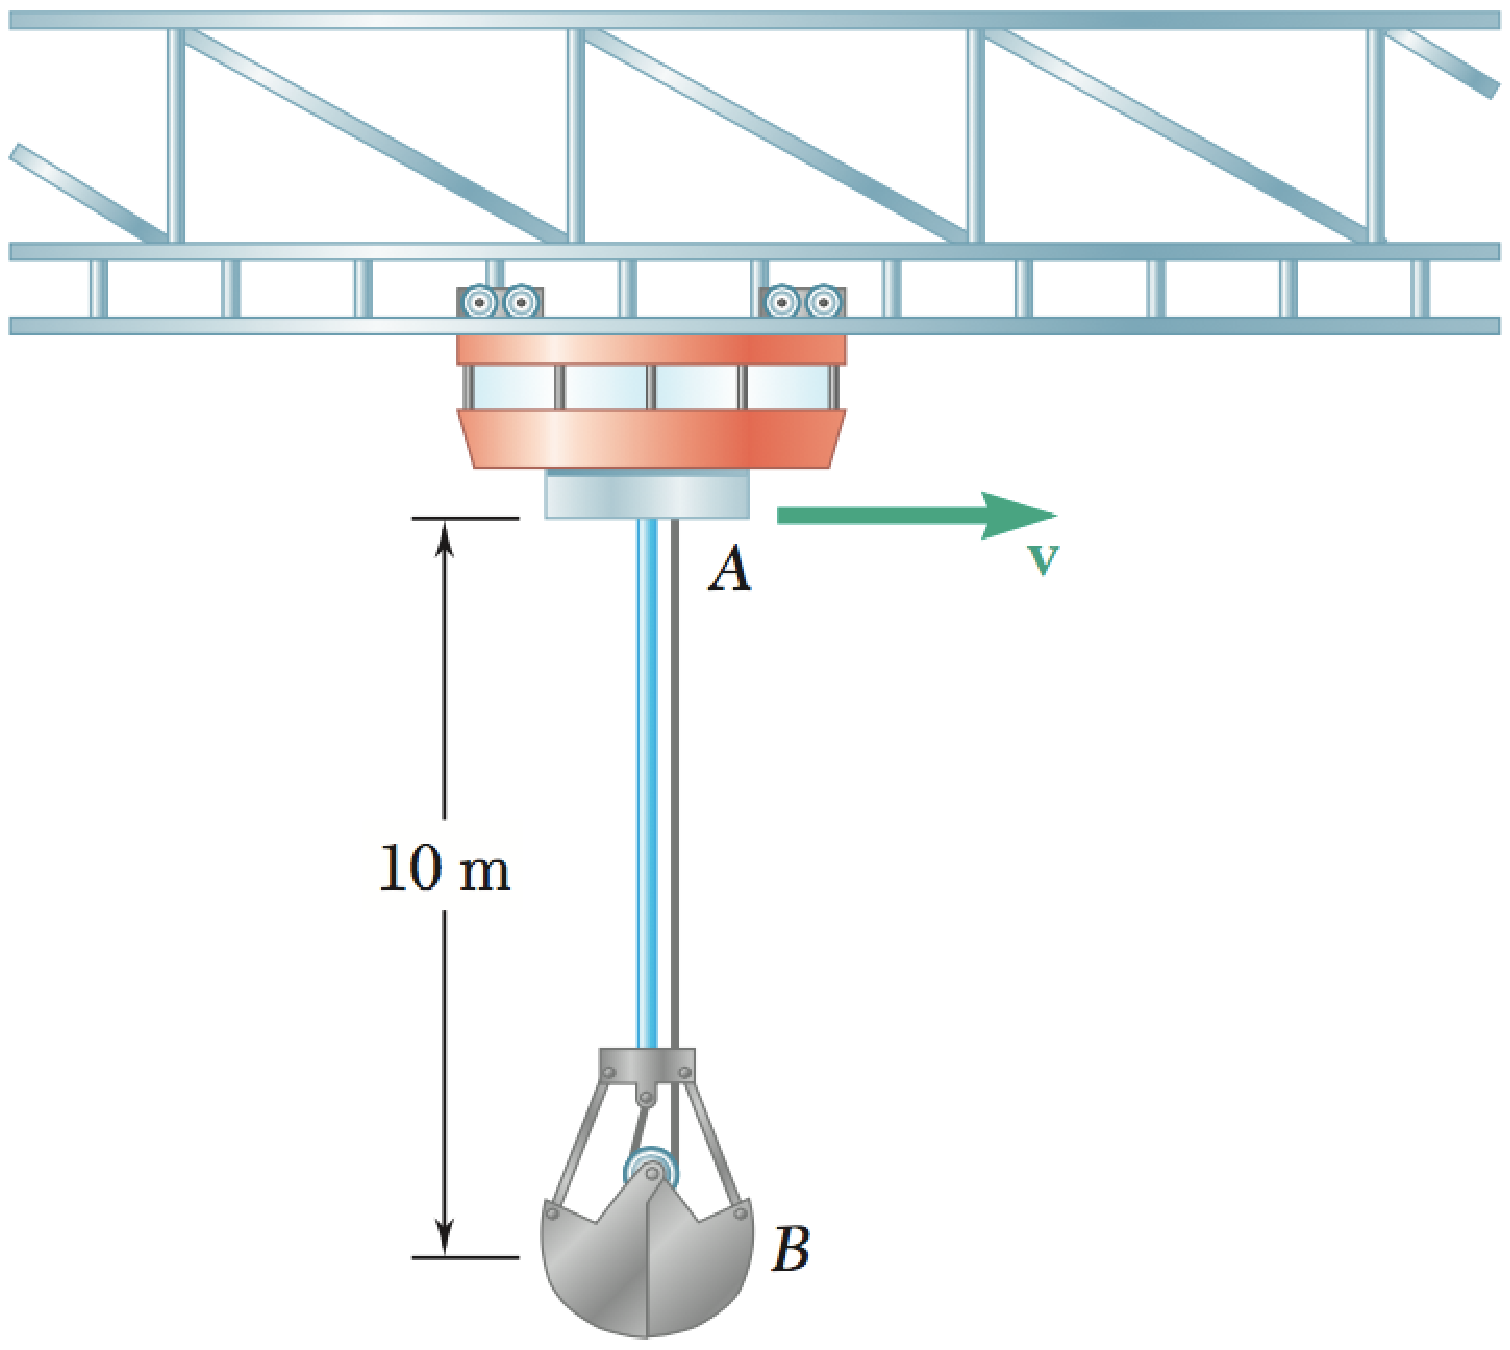
\includegraphics[width=0.4\textwidth]{./images/grua.pdf}
		\end{center}
	\end{figure}

	\item Una masa de $3 kg$ puede deslizarse sobre un riel vertical sin fricción, si esta es presionada contra un resorte en la base hasta comprimirlo $150 mm$ y despues liberada, determinar (a) la altura máxima de la masa y (b) la velocidad máxima alcanzada por la masa, suponiendo que la constante del resorte es $k = 2.6 \frac{kN}{m}$.

	\begin{figure}[h]
		\begin{center}
			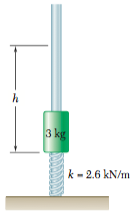
\includegraphics[width=0.2\textwidth]{./images/masa.png}
		\end{center}
	\end{figure}

	\item Un empleado de una aerolinea avienta dos maletas sucesivamente con una velocidad horizontal de $2.4 \frac{m}{s}$ a un carrito de $25 kg$, el cual inicialmente esta en reposo. (a) Sabiendo que la velocidad final del carrito es de $1.2 \frac{m}{s}$ y que la primer maleta aventada tiene una masa de $15kg$, determine la masa de la segunda maleta. (b) ¿Cual sería la velocidad final del carrito si el empleado hubiera aventado las maletas en el orden contrario?

	\begin{figure}[h]
		\begin{center}
			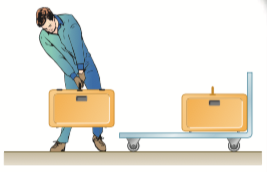
\includegraphics[width=0.4\textwidth]{./images/maletas.png}
		\end{center}
	\end{figure}

	\item Un hombre de $180 lb$ y una mujer de $120 lb$ estan parados en el mismo lado de un bote de $300 lb$, listos para lanzarse al agua, cada uno a una velocidad de $16 \frac{ft}{s}$. Determine la velocidad del bote, despues de que ambos se lanzaron de el, si (a) la mujer se lanzó primero o (b) el hombre se lanzó primero.

	\begin{figure}[h]
		\begin{center}
			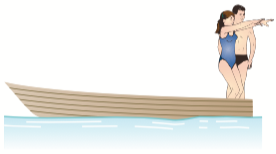
\includegraphics[width=0.4\textwidth]{./images/juntos.png}
		\end{center}
	\end{figure}

	\item Un hombre de $180 lb$ y una mujer de $120 lb$ estan parados en laods opuestos de un bote de $300 lb$, listos para lanzarse al agua, cada uno a una velocidad de $16 \frac{ft}{s}$. Determine la velocidad del bote, despues de que ambos se lanzaron de el, si (a) la mujer se lanzó primero o (b) el hombre se lanzó primero.

	\begin{figure}[h]
		\begin{center}
			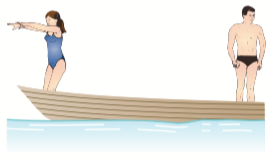
\includegraphics[width=0.4\textwidth]{./images/separados.png}
		\end{center}
	\end{figure}

	\item Una bala es disparada con una velocidad horizontal de $1500\frac{ft}{s}$ a través del bloque A con un peso de $6lb$, y se incrusta en el bloque B el cual tiene un peso de $4.95lb$. Sabiendo que los bloques adquieren velocidades de $5\frac{ft}{s}$ y $9\frac{ft}{s}$ respectivamente, determinar el peso de la bala $w_B$ y la velocidad de la bala al salir del bloque A.

	\begin{figure}[h]
		\begin{center}
			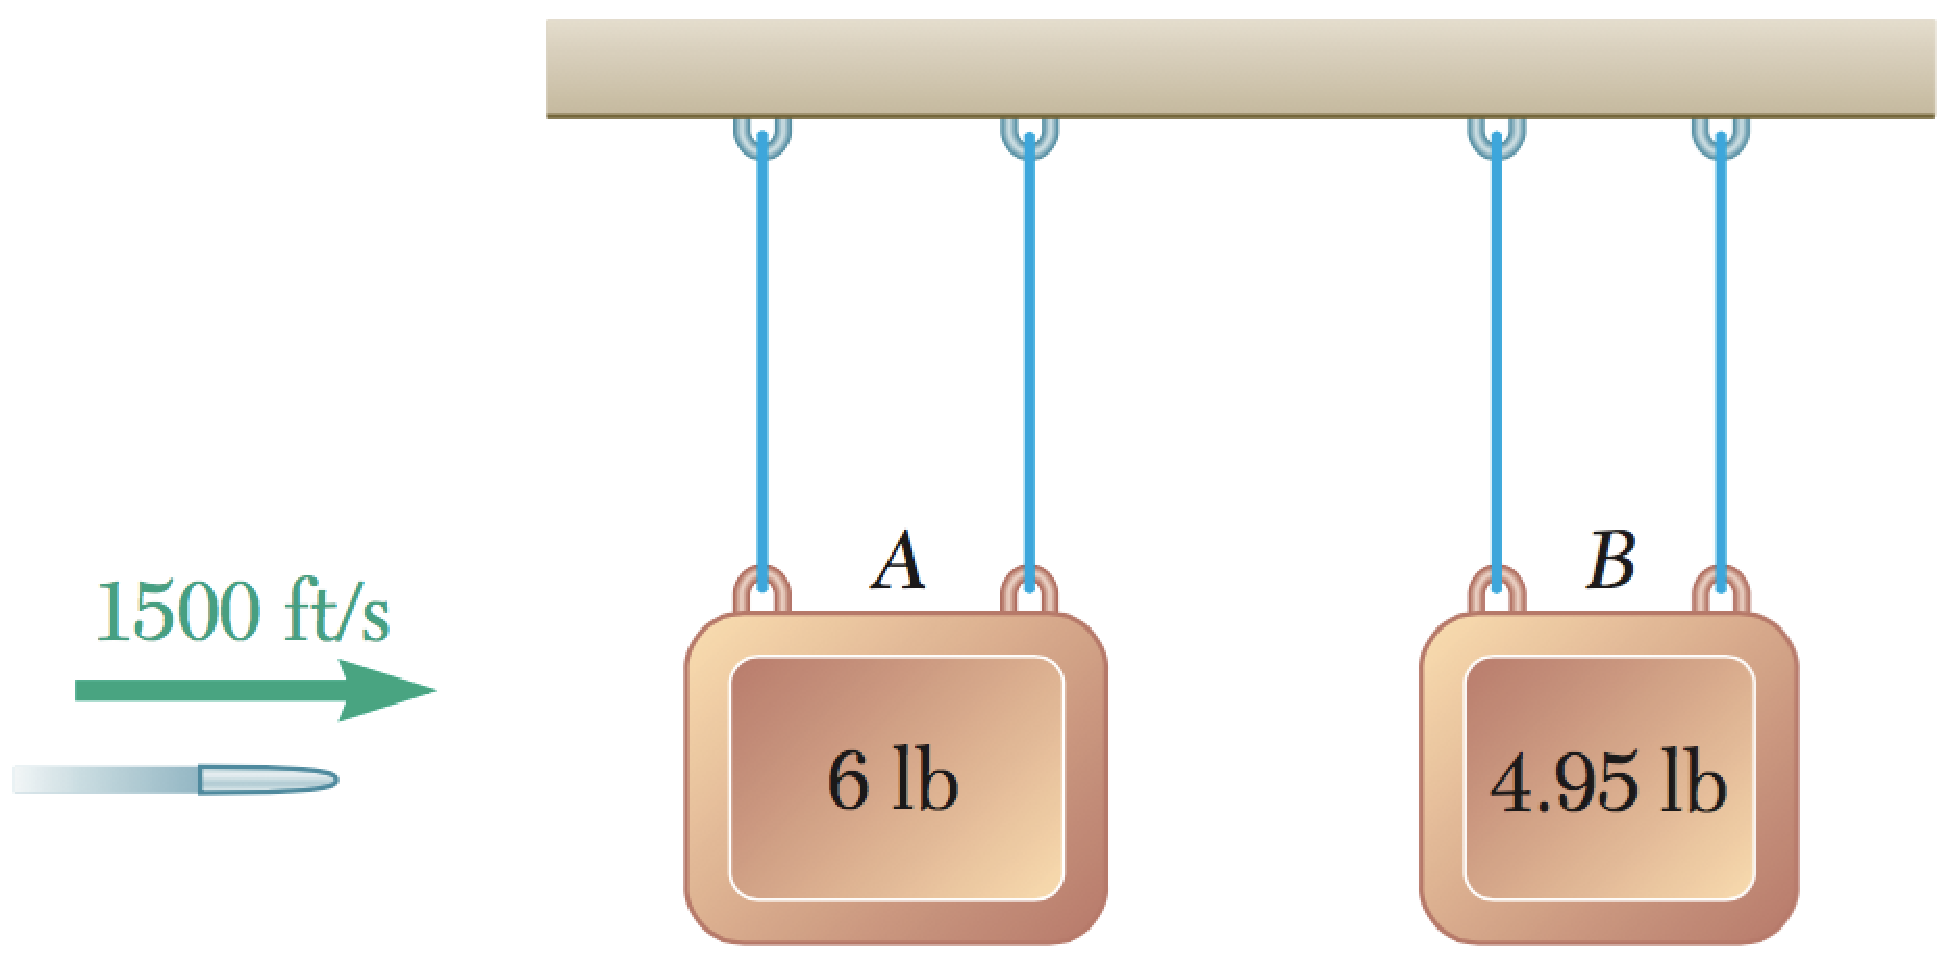
\includegraphics[width=0.4\textwidth]{./images/bala.pdf}
		\end{center}
	\end{figure}

\end{enumerate}

%-------------------------------------------------------------------------------
%	PROBLEMAS EXTRA
%-------------------------------------------------------------------------------

\section{Problemas extra}

\begin{enumerate}
	\item Una fuerza $P$ es aplicada lentamente a una placa adosada al extremo de un par de resortes como se muestra en la figura, y esta fuerza causa una deflexion $x_0$. En cada uno de los casos mostrados, obtener una expresión para la constante $k_e$ en terminos de $k_1$ y $k_2$ de tal manera que el efecto de los dos resortes sea equivalente a un tercero con esta constante $k_e$ del resorte (es decir, que este resorte tenga la misma deflexion $x_0$ debido a la misma fuerza $P$).

	\begin{figure}[h]
		\begin{center}
			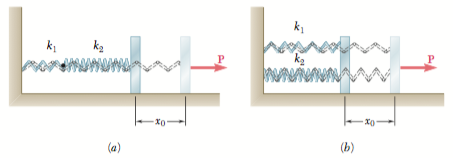
\includegraphics[width=0.8\textwidth]{./images/resortes.png}
		\end{center}
	\end{figure}

	\item Un sistema de tres particulas $A$, $B$ y $C$. Sabemos que sus masas son $m_A = 3 kg$, $m_B = 4 kg$ y $m_C = 5 kg$ y que las velocidades de las particulas, expresadas en $\frac{m}{s}$, son $v_A = -4 i + 4 j + 6 k$, $v_B = v_x i + v_y j + v_z k$, y $v_C = 2i - 6j - 4k$. Determine (a) las componentes $v_x$, $v_y$ y $v_z$ tales que el momento angular del sistema $H_O$ al rededor de $O$ sea paralelo al eje $z$ y (b) la magnitud del momento angular $H_O$.
\end{enumerate}

%-------------------------------------------------------------------------------
%	FIN DEL DOCUMENTO
%-------------------------------------------------------------------------------

\end{document}
